\chapter{Polynomials}
%%%%%%%%%%%%%%% SECTION HEADER %%%%%%%%%%%%%%%%
\rhead{4}
\lhead{Polynomials}
%%%%%%%%%%%%%%%%%%% START %%%$%%%%%%%%%%%%%%%%%
\section{Polynomials}
A  term  is  defined  as  an  expression  containing  a  number  or  the  product  of  a  number  and  one  or  more  variables  raised  to  powers. Examples of terms are
\begin{equation*}
        3x^2,\ -x^2y^3,\ 6ab,\ -10
\end{equation*}
A  polynomial  is  a  single  term  or  a  finite  sum  of  terms.  The  powers  of  the  variables  in  a  polynomial  must  be  \textbf{a positive  integer}.  For  example, $4x^3-15x^2-x+2$ is an example of polynomial. 
% ====== SECTION
\section{Monomial, binomial and trinomial}
 A polynomial with a single term is often called a \textbf{monomial}. Examples are,
 \begin{align*}
        7x,\quad -20,\quad 10y^7&
 \end{align*}
  A monomial can be a number, a variable, or the product of a number and one or more variables with whole number exponents. \\
Moreover, if a polynomial has only two terms, then it is often called a \textbf{binomial}. Such as
 \begin{align*}
        10x^4-1,\quad a^2+b,\quad -2x^2+9x
 \end{align*}
 Finally, a \textbf{trinomial} is another special type of polynomial with only three terms. Examples are 
 \begin{align*}
        10x^2+5x-1, \quad -15y^5+y^4+12y^2
 \end{align*}
 % ============== SUB SECTION
\subsection{Degree of a polynomial}
The degree of a polynomial is the highest power of the variable in the polynomial. Examples:
\begin{align*}
    4x^3−15x^2+x−2& & &\text{Degree = 3}\\
    7w−w^2& &   &\text{Degree = 2}\\
    10y^7-100y^2-1000&  &   &\text{Degree = 7}
\end{align*}
 \begin{nt}
     The degree of a polynomial consisting of a single number is zero. For instance, 7 is a polynomial with degree of 0.
 \end{nt}
 \subsection{Leading coefficient and the constant term}
 The number preceding the variable in each term is called the coefficient of that variable or the coefficient of that term. For example, in $4x^3−15x^2+x−2$ 
 \begin{align*}
     \text{Coefficient of $x^3$} & = 4 \\
     \text{Coefficient of $x^2$} & = -15 \\
     \text{Coefficient of $x\ $} & = 1
 \end{align*}
 \begin{nt}
    In our example, the coefficient of $x$ is 1 because $x=1.x$. So if there is no number in front of the variable, the coefficient is 1.
 \end{nt}
 The coefficient of the variable with the highest exponent is called
 leading coefficient and the number without variable is called the constant term. Considering $-20x^6+23x^4+2x^3-10x+44$, for example, we have
 \begin{align*}
    \text{Leading coefficient} & = -20 \\
    \text{Constant term} &= 44
 \end{align*}
 % ========== SECTION =============
 \section{FOIL method}
 When you are multiplying two binomials, you need to use FOIL method.
 The word FOIL is an acronym for the four terms of the product:
\begin{itemize}
    \item \textcolor{red}{F}irst ("first" terms of each binomial are multiplied together)
    \item \textcolor{red}{O}uter ("outside" terms are multiplied—that is, the first term of the first binomial and the second term of the second)
    \item \textcolor{red}{I}nner ("inside" terms are multiplied—second term of the
    first binomial and first term of the second)
    \item \textcolor{red}{L}ast ("last" terms of each binomial are multiplied) 
\end{itemize}
\begin{figure*}[ht]
    \centering
    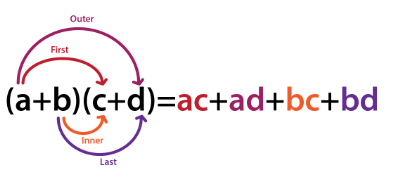
\includegraphics[width=7cm]{pics/foil-method-formula.png}
    \label{fig:foil}
\end{figure*}
% ========== EXAMPLE 1
\begin{exa}
    Simplify $(2x+1)(x-3)$
\end{exa}
Using the FOIL method, we get
\begin{align*}
    (2x+1)(x-3)& \\
    (2x)(x)+(2x)(-3)+(1)(x)+(1)(-3)& \\
    2x^2-6x+x-3&    &   &\text{Combine like terms}\\
    2x^2-5x-3& &&\text{Our solution}
\end{align*}
% ======== Example 2
\begin{exa}
    Simplify $(4x+y)(3x-2y)$.
\end{exa}
Use the FOIL method, we'll get
\begin{align*}
    (4x+y)(3x-2y)&  &&\\
    (4x)(3x)+(4x)(-2y)+(y)(3x)+(y)(-2y)& &&\\
    12x^2-8xy+3yx-2y^2& &&\text{Combine like terms}\\
    12x^2-5xy-2y^2 &    &&\text{Our answer}
\end{align*}
% ==========
In previous example, some students like to think of the FOIL method as distributing the first term $4x$ through the $(3x − 2y)$ and distributing the second term $7y$ through the $(3x − 2y)$. Thinking about FOIL in this way makes it possible to extend this method to problems with more terms.
% ====== EXAMPLE 3
\begin{exa}
    Simplify $(2x-3)(4x^2-7x+1)$.
\end{exa}
\begin{align*}
    (2x-3)(4x^2-7x+1)&  &&\text{Distribute $2x$ and $-3$}\\
    {\scriptstyle (2x)(4x^2)+(2x)(-7x)+(2x)(1)+(-3)(4x^2)+(-3)(-7x)+(-3)(1)}& &&\\
    8x^3-14x^2+2x-12x^2+21x+3&    &&\text{Combine like terms}\\
    8x^3-26x^2+23x+3&   &&\text{Our answer}
\end{align*}
